\documentclass[t]{beamer}
\usetheme{Madrid}
\usecolortheme{default}

\usepackage{booktabs} % Untuk garis \toprule, \midrule, \bottomrule
\usepackage{graphicx} % Untuk \resizebox
\usepackage{tikz}
\usetikzlibrary{trees}
\usepackage{booktabs}
\usepackage{xcolor}
\usepackage{tabularx}
\usepackage{ragged2e} % Untuk perataan teks yang lebih rapi

\title[Visualisasi Data - Pertemuan 5]{Marks and Channels}

\author{Ahmad Luky Ramdani}
\subtitle{Matakuliah Visualisasi Data (Data visualization)}
\author[Ahmad Luky Ramdani]{Ahmad Luky Ramdani \and Ira Safitri \and Dimas Dwi Randa}
\institute[ITERA]
{
  Program Studi Data Sains\\
  Fakultas Sains \\
  Institut Teknologi Sumatera
}

\date{Bandung, \today}
\begin{document}
\frame{\titlepage}


% === 
\begin{frame}{Gambaran Umum (\textit{The Big Picture})}
    Dalam desain visualisasi data, menerjemahkan data abstrak menjadi representasi visual bergantung pada kombinasi dua elemen fundamental:
    \vspace{0.5cm}
    \begin{itemize}
        \item \textbf{Marks} (Tanda/Geometri Dasar)
        \item \textbf{Channels} (Saluran Visual)
    \end{itemize}
    \vspace{0.5cm}
    \textit{The Big Picture} dari bab ini adalah memahami bagaimana menghubungkan tipe data dengan tipe saluran visual yang tepat agar informasi tersampaikan secara akurat dan tidak menyesatkan persepsi manusia.
\end{frame}

% Slide 3: Marks
\begin{frame}{Marks: Elemen Geometri Dasar}
    \textit{Marks} adalah representasi fisik atau elemen grafis dasar yang mewakili satu baris data (\textit{item}) atau relasi antar data (\textit{link}).
    \vspace{0.3cm}

    Marks diklasifikasikan berdasarkan dimensi spasialnya:
    \begin{itemize}
        \item \textbf{0D (Point/Titik):} Tidak memiliki dimensi ukuran. Hanya menunjukkan lokasi. \textit{(Contoh: Titik pada scatterplot)}
        \vspace{0.2cm}
        \item \textbf{1D (Line/Garis):} Memiliki panjang tetapi lebar diabaikan. Menunjukkan koneksi/lintasan. \textit{(Contoh: Garis tren pada line chart)}
        \vspace{0.2cm}
        \item \textbf{2D (Area/Bidang):} Memiliki panjang dan lebar (luasan) yang mengisi ruang. \textit{(Contoh: Poligon batas provinsi pada peta)}
    \end{itemize}
\end{frame}

% Slide 4: Intro Channels
\begin{frame}{Channels: Pengendali Tampilan Visual}
    \textit{Channels} adalah variabel visual yang mengontrol dan memodifikasi penampilan dari \textit{Marks}. 
    \vspace{0.5cm}

    Channels digunakan untuk menyandikan (\textit{encode}) atribut data ke dalam mark. Berdasarkan jenis data yang diwakilinya, saluran visual terbagi menjadi dua:
    \vspace{0.3cm}
    \begin{enumerate}
        \large
        \item \textbf{Magnitude Channels} \\ \normalsize (Untuk Data Kuantitatif \& Ordinal)
        \vspace{0.2cm}
        \item \textbf{Identity Channels} \\ \normalsize (Untuk Data Kategorikal)
    \end{enumerate}
\end{frame}

% Slide 5: Magnitude Channels
\begin{frame}{Magnitude Channels}
    \textbf{Konteks:} Untuk Data Kuantitatif \& Ordinal
    \vspace{0.2cm}
    
    Digunakan untuk menjawab pertanyaan \textbf{``Seberapa banyak?''} (\textit{How much?}). Mata manusia secara alami dapat mengurutkan nilai pada saluran ini dari yang terkecil hingga terbesar.
    \vspace{0.3cm}

    \textbf{Contoh (Dari yang paling akurat ke kurang akurat):}
    \begin{itemize}
        \item Posisi pada sumbu referensi yang sama (seperti \textit{Bar Chart})
        \item Posisi pada sumbu yang tidak disejajarkan
        \item Panjang (\textit{Length} / ukuran 1D)
        \item Sudut atau Kemiringan (\textit{Tilt/Angle})
        \item Luas Area (\textit{Area} / ukuran 2D)
        \item Kecerahan/Intensitas Warna (\textit{Color Luminance/Saturation})
    \end{itemize}
\end{frame}

% Slide 6: Identity Channels
\begin{frame}{Identity Channels}
    \textbf{Konteks:} Untuk Data Kategorikal
    \vspace{0.2cm}

    Digunakan untuk menjawab pertanyaan \textbf{``Ini apa?''} atau \textbf{``Di mana?''} (\textit{What? / Where?}). Tidak ada urutan besaran implisit; murni untuk membedakan identitas antar kelompok data.
    \vspace{0.3cm}

    \textbf{Contoh Channel:}
    \begin{itemize}
        \item Wilayah Spasial (\textit{Spatial Region})
        \item Rona Warna (\textit{Color Hue} -- misalnya: merah, biru, kuning)
        \item Bentuk (\textit{Shape} -- misalnya: lingkaran, segitiga, persegi)
        \item Pola pergerakan (\textit{Motion})
    \end{itemize}
\end{frame}

% Slide 7: The Golden Rules
\begin{frame}{Dua Prinsip Emas (\textit{The Golden Rules})}
    Untuk menghindari disinformasi visual, perancangan Marks dan Channels wajib mematuhi dua aturan baku:
    \vspace{0.3cm}
    
    \begin{enumerate}
        \item \textbf{Prinsip Ekspresi (\textit{Expressiveness}):} \\
        Visualisasi harus mengekspresikan informasi yang ada dalam atribut data, tidak kurang dan tidak lebih. Tipe \textit{channel} \textbf{harus cocok} dengan tipe data.
        \vspace{0.4cm}
        \item \textbf{Prinsip Keefektifan (\textit{Effectiveness}):} \\
        Atribut data yang paling penting secara bisnis harus disandikan menggunakan \textit{channel} yang menduduki peringkat tertinggi dalam hierarki persepsi visual manusia (Misal: pakai \textit{Posisi/Panjang}, bukan \textit{Warna/Luas}).
    \end{enumerate}
\end{frame}

% === 

\begin{frame}{Marks vs. Channels}
	\begin{itemize}
		\item Marks adalah kanvas/objek fisiknya atau Bentuk Geometri Dasar
			\begin{itemize}
				\item Elemen dasar yang mewakili satu baris data (item) atau hubungan antar data (link)
				\item Terdiri dari:
				\begin{itemize}
					\item 0D - Point (Titik): Tidak punya ukuran intrinsik, hanya penanda lokasi. Contoh: Titik pada Scatterplot.
					\item 1D - Line (Garis): Memiliki panjang, tidak punya lebar. Contoh: Garis pada Line Chart atau garis penghubung pada Network Graph.
					\item 2D - Area (Bidang/Luasan): Memiliki panjang dan lebar untuk mengisi ruang. Contoh: Irisan pada Pie Chart atau batas negara pada Peta.
				\end{itemize}
			\end{itemize}
		\item Channels adalah kuas/cat yang mengubah tampilan objek tersebut atau Saluran Visual
		\begin{itemize}
			\item Cara kita memodifikasi/mengubah tampilan Marks untuk menyandikan (encode) nilai dari atribut data
			\item Anda punya Mark berupa Titik (0D). Anda bisa mengubah Posisi titik tersebut (X dan Y), mengubah Warna titiknya, atau mengubah Ukuran titiknya. Posisi, warna, dan ukuran inilah yang disebut Channels.
		\end{itemize}
	\end{itemize}

\end{frame}

% === 

\begin{frame}{Marks for items}
	\begin{itemize}
		\item basic geometric elements
		\item 3D volumes, not covered in this course
	\end{itemize}

	\begin{center}
		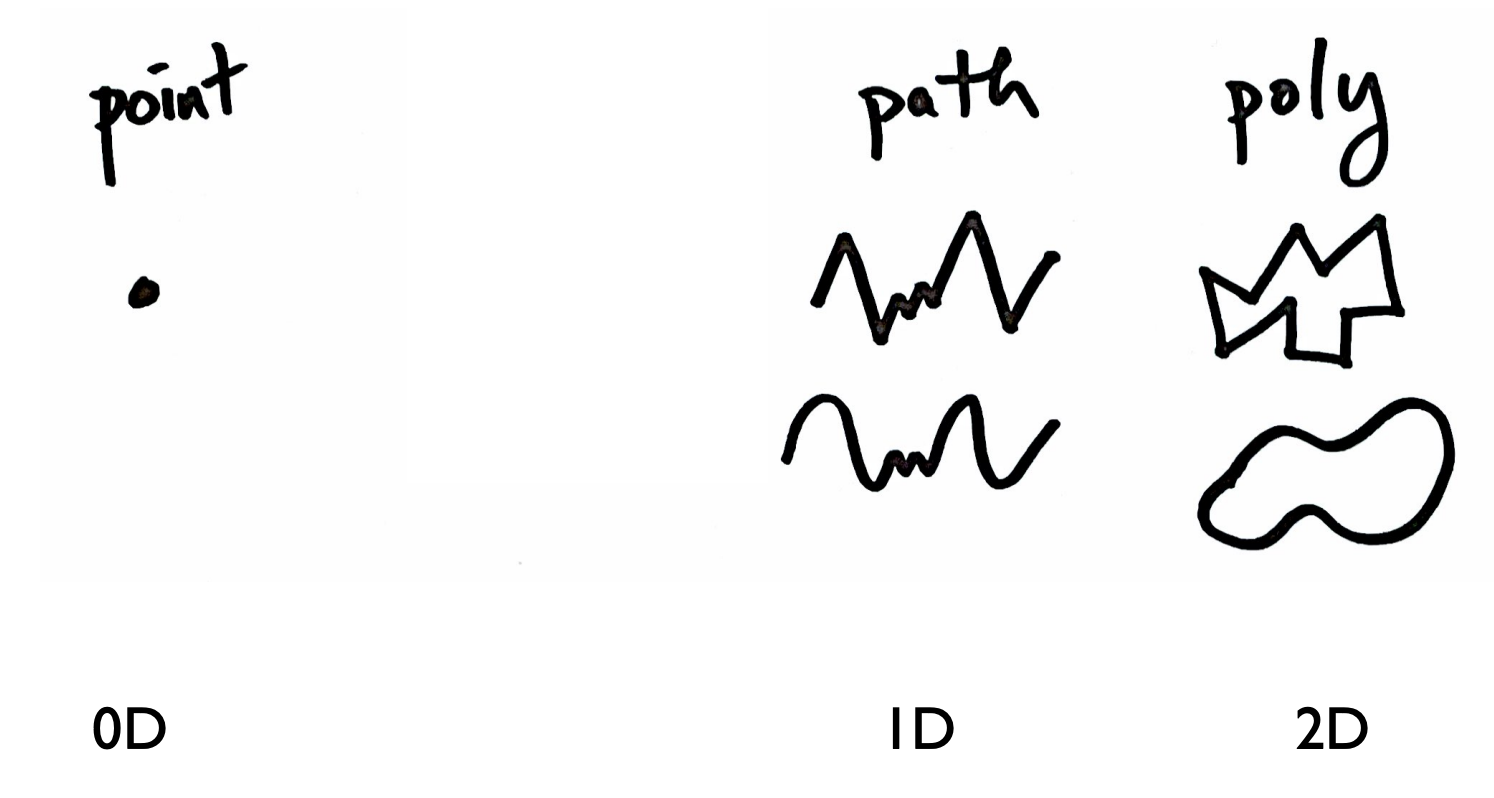
\includegraphics[width=0.8\textwidth]{image.png}
	\end{center}
\end{frame}

% === 
\begin{frame}{Marks for items}
	\begin{itemize}
		\item basic geometric elements
	\end{itemize}
	\begin{center}
		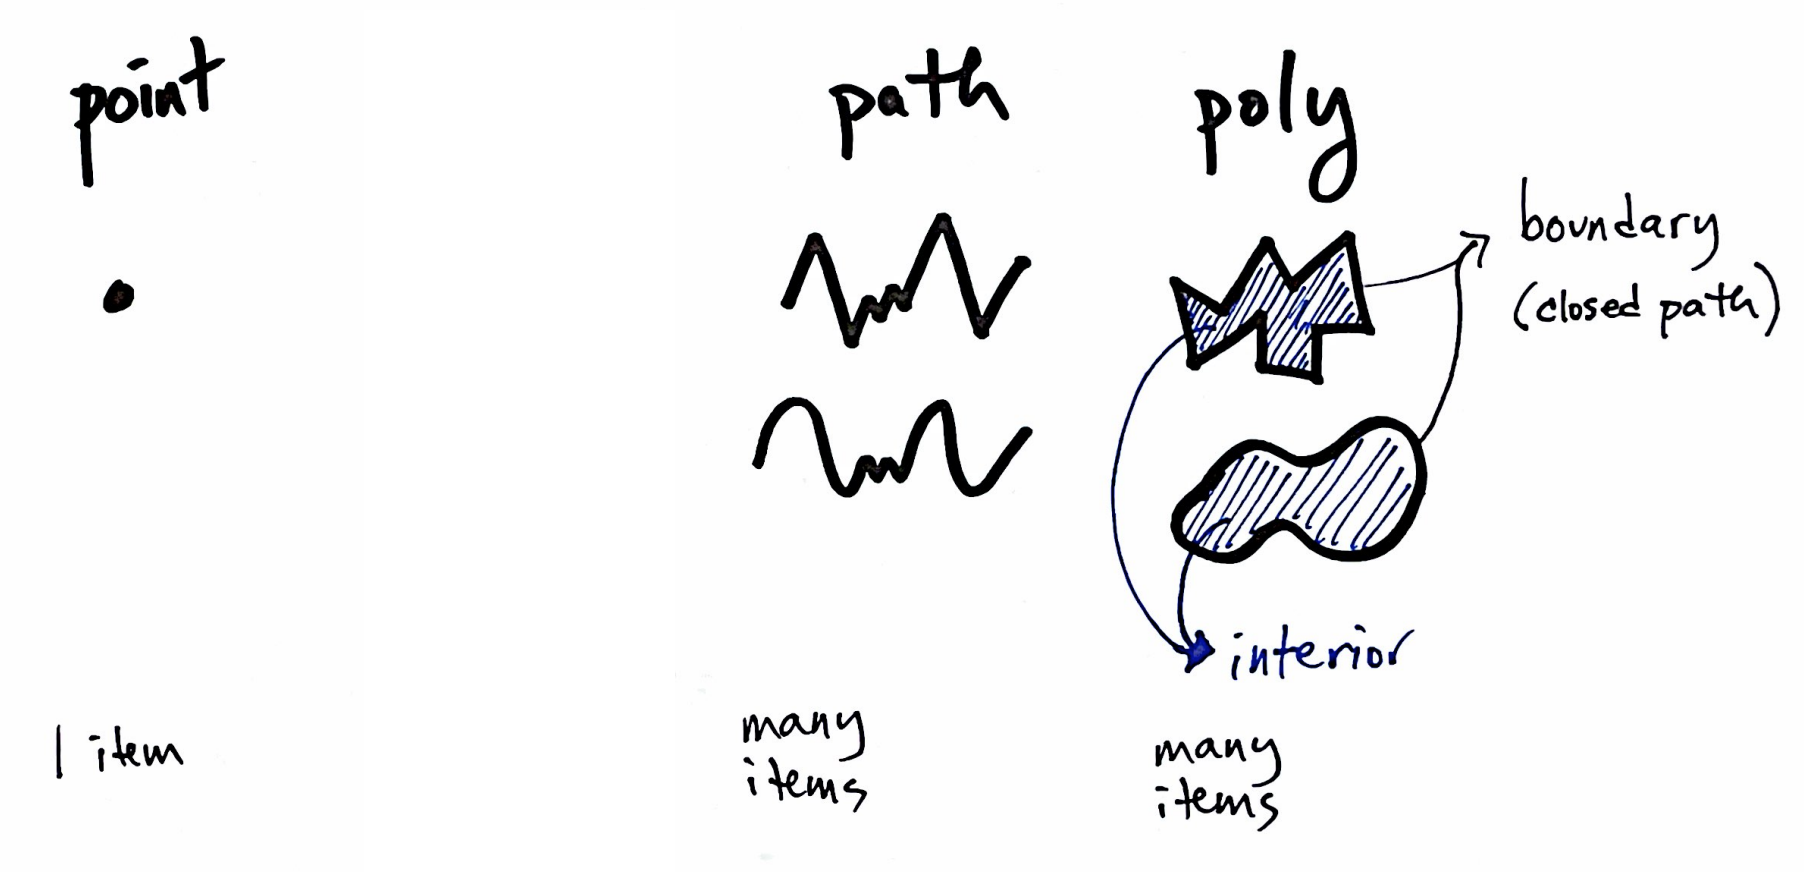
\includegraphics[width=0.8\textwidth]{image2.png}
	\end{center}
\end{frame}

% === 

\begin{frame}{Marks for items}
	\begin{itemize}
		\item basic geometric elements
	\end{itemize}
	\begin{center}
		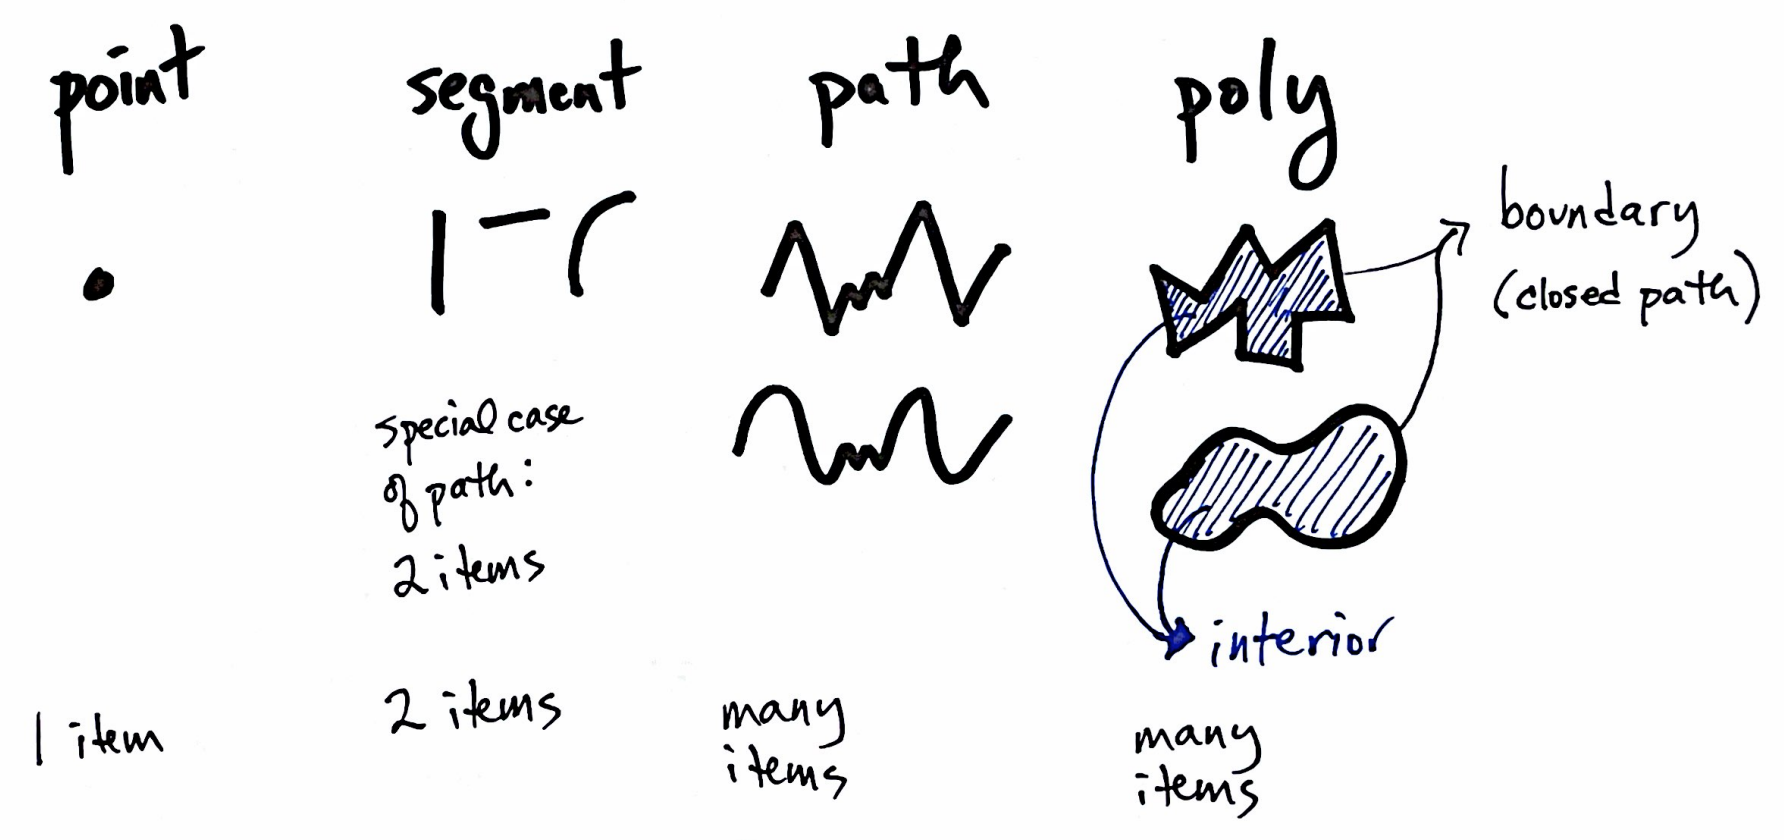
\includegraphics[width=0.8\textwidth]{image3.png}
	\end{center}
\end{frame}

% === 

\begin{frame}{Dua Tipe Channels: Magnitude vs. Identity}
	\begin{itemize}
		\item Magnitude Channels (Untuk Data Kuantitatif \& Ordinal)
		\begin{itemize}
			\item Menjawab pertanyaan: Seberapa banyak? / Mana yang lebih besar?
			\item Bisa diurutkan secara logis oleh mata.
			\item Contoh: Posisi pada sumbu (paling akurat), Panjang garis, Kemiringan (sudut), Luas area, dan Saturasi warna (terang ke gelap).
		\end{itemize}
		\item Identity Channels (Untuk Data Kategorikal)
		\begin{itemize}
			\item Menjawab pertanyaan: "Ini apa?" atau "Di mana lokasinya?"
			\item Tidak bisa diurutkan (kita tidak bisa bilang merah lebih besar dari biru).
			\item Contoh: Bentuk (lingkaran vs kotak), Color Hue (merah, biru, hijau), dan Region spasial (kiri vs kanan).
		\end{itemize}
	\end{itemize}
\end{frame}

% === 

\begin{frame}{Dua Prinsip Desain (The Golden Rules)}
	\begin{itemize}
		\item The Expressiveness Principle (Prinsip Ekspresi)
		\begin{itemize}
			\item Visualisasi harus menceritakan kebenaran data, tidak kurang dan tidak lebih. Tipe Channel harus cocok dengan tipe Data.
			\item Pelanggaran umum: Menggunakan ukuran/luas lingkaran (Magnitude) untuk membedakan nama merk mobil (Identity). Orang akan mengira mobil dengan lingkaran besar lebih unggul, padahal itu cuma nama.
			\item Contoh: Menggunakan warna untuk menunjukkan perbedaan kategori, tapi ternyata warna itu mewakili nilai kuantitatif (misalnya, semakin gelap warnanya, semakin tinggi nilainya). Orang akan bingung apakah warna itu menunjukkan kategori atau nilai.
		\end{itemize}
	\end{itemize}
\end{frame}

% === 

\begin{frame}{Dua Prinsip Desain (The Golden Rules)}
	\begin{itemize}
		\item The Effectiveness Principle (Prinsip Keefektifan)
		\begin{itemize}
			\item Visualisasi harus menggunakan Channel yang paling efektif untuk menyampaikan informasi. Untuk data kuantitatif, gunakan Channel Magnitude yang paling akurat (misalnya, posisi pada sumbu). Untuk data kategorikal, gunakan Channel Identity yang paling mudah dibedakan (misalnya, warna hue).
			\item Pelanggaran umum: Menggunakan warna hue (Identity) untuk menunjukkan perbedaan nilai kuantitatif (Magnitude). Orang akan kesulitan membandingkan nilai-nilai tersebut karena warna tidak diurutkan secara logis.
			\item Contoh: 1). Menggunakan panjang garis (Magnitude) untuk menunjukkan perbedaan kategori (Identity). Orang akan mengira kategori dengan garis lebih panjang lebih penting, padahal itu cuma nama. 2). Jika membandingkan "Total Penjualan" adalah tugas utama (Task), gunakan Channel Posisi/Panjang (seperti Bar Chart). Jangan gunakan gradasi warna, karena mata manusia sangat buruk dalam menghitung selisih angka murni hanya dari melihat tingkat kegelapan warna.
		\end{itemize}
	\end{itemize}
\end{frame}

% === 

% --- Final page ---
\begin{frame}[c]
    \centering
    \Huge{Terima Kasih} % 
    
    \vspace{1.5cm}
    \normalsize
    \textbf{Ahmad Luky Ramdani} \\ % 
    \href{mailto:ahmadluky@sd.itera.ac.id}{ahmadluky@sd.itera.ac.id} % 
\end{frame}




\end{document}
